\documentclass{beamer}

\mode<presentation> {
    \usetheme{Warsaw}
    %\usecolortheme{beaver}
    \setbeamertemplate{navigation symbols}{}
    %\setbeamercolor{item}{fg=darkred}
}

\usepackage[french]{babel}
\usepackage[utf8x]{inputenc}
\usepackage{graphicx}

\usepackage{listings}

\lstset{
    language=C,
    %numbers=left,
    stepnumber=1,
    numbersep=5pt,
    backgroundcolor=\color{white},
    showspaces=false,
    showstringspaces=false,
    showtabs=false,
    tabsize=2,
    captionpos=b,
    breaklines=true,
    breakatwhitespace=true,
    basicstyle=\fontsize{7}{11}\ttfamily,
    keywordstyle=\bfseries\color{red!40!black},
    commentstyle=\itshape\color{gray},
    stringstyle=\color{orange},
}

\title[Presentation SEA]{Projet 4IF : Raspberry PI}
\author{H4104 - équipe Dragibus}
\institute{INSA de Lyon}
\date{Vendredi 13 décembre 2013}

\begin{document}

\begin{frame}
    \titlepage
\end{frame}

\begin{frame}
    \frametitle{Introduction}

    % TODO
\end{frame}

\begin{frame}
    \frametitle{Sommaire}
    \tableofcontents
\end{frame}

\section{Synchronisation}

\begin{frame}
    \frametitle{Synchronisation des processus}

    \begin{center}
        \huge conception en couches
    \end{center}

    \begin{enumerate}
        \item<2-> \textbf{sémaphore}: compteur à intervalle bloquant le
            processus appelant (opération +1/-1) s'il cause un dépassement
        \item<3-> \textbf{mutex}: sémaphore de 0 à 1, permettant un
            acquire/release, uniquement par un processus à la fois
        \item<4-> \textbf{pipe}: FIFO avec mutex associé
    \end{enumerate}
\end{frame}

\begin{frame}[fragile]
    \frametitle{Problème de synchronisation (résolu)}

    \begin{lstlisting}[caption=Opération atomique sur un sémaphore]
        void sem_op(struct sem_s * sem, struct sem_op_s * op) {
            DISABLE_IRQ();

            /* operation sur le semaphore */

            ENABLE_IRQ();
        }
    \end{lstlisting}
\end{frame}

\section{Ordonnancement sur mini-OS}

\begin{frame}
    \frametitle{Les problématiques d'ordonnancement}
    \begin{center}
        \huge Objectifs
    \end{center}
    \begin{itemize}
        \item<2-> rapide
        \item<3-> automatique
        \item<4-> équitable
    \end{itemize}
\end{frame}

\begin{frame}
    \frametitle{Ordonnancements mis en place}
    \begin{itemize}
        \item<2-> préemptif
        \item<3-> collaboratif
        \item<4-> prioritaire
    \end{itemize}
\end{frame}

\begin{frame}
    \frametitle{Critique des différents ordonnancements}
    \begin{itemize}
        \item préemptif: aucune distinction entre les différents processus
        \item collaboratif: manque d'automatisme (\textbf{yield()} nécessaire)
        \item prioritaire: problématique du \emph{bon} ordre
    \end{itemize}
\end{frame}

\begin{frame}
    \frametitle{Politique d'ordonnancement choisie}
    \begin{center}
        \huge combinaison
    \end{center}
\end{frame}

\begin{frame}[fragile]
    \frametitle{Ordonnancement d'une tâche}
    \begin{lstlisting}[caption=Représentation structurelle d'un processus]
        struct task {
            /* Etat de la tache */
            int state, needs_reschedule;

            /* Politique d'ordonnancement */
            int policy;

            /* Priorite */
            time_t priority, realtime_priority,
                current_priority;

            /* Processus suivant/precedent */
            struct task * next, * prev;

            /* contexte, informations temporelles, etc... */
        };
    \end{lstlisting}
\end{frame}

\begin{frame}
    \frametitle{Ordonnancement d'une tâche}

    % TODO
\end{frame}

\begin{frame}
    \frametitle{Performances du mini-OS}

    % TODO
\end{frame}

\section{Ordonnancement sur Linux}

\begin{frame}
    \frametitle{Problématiques d'ordonnancement sous Linux}

    % TODO
\end{frame}

\begin{frame}
    \frametitle{Exemple: short vs long}

    \begin{center}
        \huge
        Concurrence entre deux processus ayant des politiques d'ordonnancement
        différentes
    \end{center}
\end{frame}

\begin{frame}[fragile]
    \frametitle{Exemple: short vs long}

    \begin{lstlisting}[caption=processus long]
        void run_long_process {
            sched_process(NORMAL, LONG_PRIORITY);
            for (size_t i = 0; i < LONG_NB_COMPUTATIONS; i++) {
                printf_safe("LONG\n");
                /* calcul long */
            }
        }
    \end{lstlisting}
\end{frame}

\begin{frame}[fragile]
    \frametitle{Exemple: short vs long}

    \begin{lstlisting}[caption=processus court]
        void run_short_process {
            sched_process(REAL_TIME, SHORT_PRIORITY);
            for (;;) {
                printf_safe("SHORT\n");
                /* calcul court */
            }
        }
    \end{lstlisting}
\end{frame}

\begin{frame}
    \frametitle{Exemple: short vs long}

    \begin{center}
        \begin{figure}
            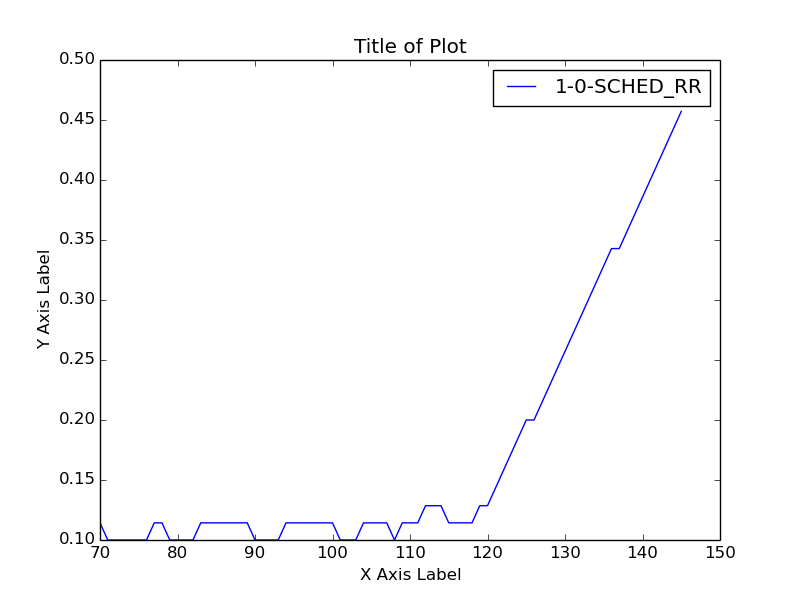
\includegraphics[scale=0.3]{../../short_vs_long/figures/1-0-SCHED_RR.png}
            \caption{Court bas, long normal}
        \end{figure}
    \end{center}
\end{frame}

\begin{frame}
    \frametitle{Exemple: short vs long}

    \begin{center}
        \begin{figure}
            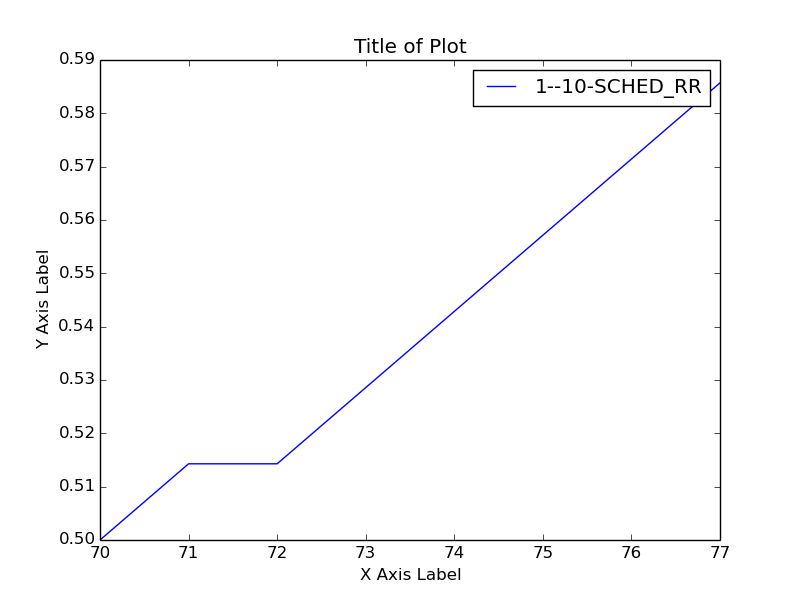
\includegraphics[scale=0.3]{../../short_vs_long/figures/1--10-SCHED_RR}
            \caption{Court bas, long haut}
        \end{figure}
    \end{center}
\end{frame}

\begin{frame}
    \frametitle{Exemple: short vs long}

    \begin{center}
        \begin{figure}
            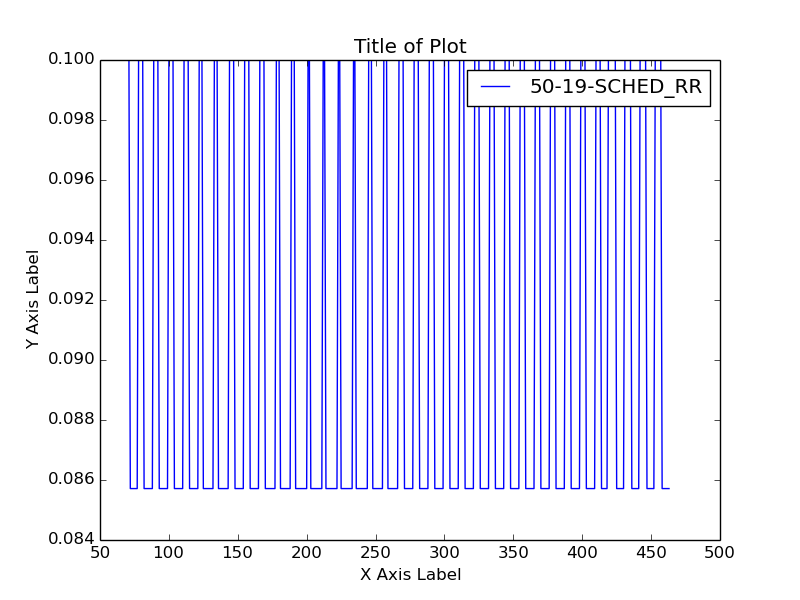
\includegraphics[scale=0.3]{../../short_vs_long/figures/50-19-SCHED_RR.png}
            \caption{Court moyen, long bas}
        \end{figure}
    \end{center}
\end{frame}

\begin{frame}
    \frametitle{Exemple: short vs long}

    \begin{center}
        \begin{figure}
            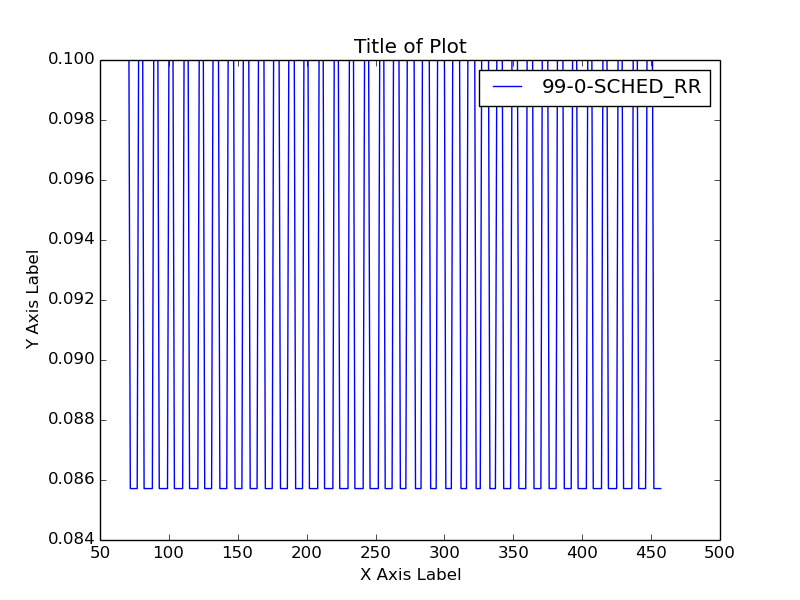
\includegraphics[scale=0.3]{../../short_vs_long/figures/99-0-SCHED_RR.png}
            \caption{Court haut, long moyen}
        \end{figure}
    \end{center}
\end{frame}

\begin{frame}
    \frametitle{Compromis CPU / Requêtes IO}

    % TODO
\end{frame}

\section{Algorithmes et problématiques}

\begin{frame}[fragile]
    \frametitle{Analyse des algorithmes}

    \begin{lstlisting}[caption=Choix de la prochaine tâche à exécuter]
        struct task * choose_next_task() {
            struct task * next = NULL;
            for (unsigned int i = 2*MAX_PRIO - 1 ; i >= 0 ; i--) {
                if (realtime_active_tasks->queue[i]) {
                    return realtime_active_tasks->queue[i];
                } else if (!next && active_tasks->queue[i]) {
                    next = active_tasks->queue[i];
                }
            }
            return next;
        }
    \end{lstlisting}
\end{frame}

\begin{frame}[fragile]
    \frametitle{Analyse des algorithmes}

    \begin{lstlisting}[caption=Détection de l'activité d'une tâche (IO/CPU)]
        void detect_task_activity() {
            struct task_struct * prev = current_task;
            if (prev != &idle_task && prev->state == TASK_READY && prev->policy & SCHED_YIELD) {
                size_t k = prev->current_priority;
                active_tasks->queue[k] = queue_del(active_tasks->queue[k], prev);
                active_tasks->queue[0] = queue_push(active_tasks->queue[0], prev);
                prev->policy &= ~SCHED_YIELD;
                prev->need_reschedule = 0;
                prev->current_priority = 0;
            }
        }
    \end{lstlisting}
\end{frame}

\begin{frame}
    \frametitle{Problèmes divers rencontrés}

    \uncover<1->{
        \begin{block}{Problème}
            Aucune sortie visible n'est disponible pour déboguer les
            fonctionnalités du kernel.
        \end{block}
    }

    \uncover<2->{
        \begin{block}{Solution}
            Nous traduisons les messages par un clignotement de la LED disponible,
            suivant un \textbf{code morse}.
        \end{block}
    }
\end{frame}

\end{document}
